\documentclass[a4paper, 12pt]{article}
\usepackage[utf8]{inputenc}
\usepackage[english]{babel}
\usepackage{apacite}
\usepackage{fancyhdr}
\usepackage{geometry}
\usepackage[hidelinks]{hyperref}
\usepackage{amsmath, amsthm, amssymb, amsfonts}
\usepackage{marginnote}
\geometry{ left=20mm, right=20mm, top=20mm,bottom=20mm, marginparwidth=35mm}
\usepackage{graphicx}
\usepackage{caption}
\usepackage{subcaption}
\usepackage{multicol}
\usepackage{natbib}
\bibliographystyle{apacite}
\graphicspath{ {C:/Users/81804/Desktop/readingSummary/figtab}}

\renewcommand{\vec}[1]{\mathbf{#1}}
\linespread{1}

\newcommand{\R}{\mathbb{R}}
\newcommand{\N}{\mathbb{N}}

\newcommand\fnote[1]{\captionsetup{font=small}\caption*{ #1}}

\begin{document}
\pagestyle{fancy}
\setlength{\parindent}{5ex}
\setlength{\columnseprule}{0.5pt}

\title{Summary:
\\Social Insurance and the Marriage Market \\
\large Journal of Political Economy, 2020, vol. 128, no. 1 \\
\large Petra Persson
}
\author{\url{https://github.com/s-saisw/studyGroup}}
\date{\today}
\maketitle

\rhead{Social Insurance and the Marriage Market}
\lhead{}

\section{Introduction}
\begin{itemize}
\item Swedish government eliminates a survivor insurance.
\begin{itemize}
\item Sweden used to provide survivors insurance to a female widow. The widow was granted a lifetime benefits upon her husband's death. Cohabiting partners or divorcees were not eligible.
\item More specifically, couples were eligible to survivors insurance if they
\begin{enumerate}
\item had a joint child and married before December 31, 1989 
\item had no joint child before December 31, 1989 but married before December 31, 1984
\end{enumerate}
\item The reform was discussed for the first time in the Parliament in June, 1988. This date was treated as reform announcement.
\end{itemize}
\item (Broad) Research Question: How does the new institution setting affect the volume and nature of marriage contract?
\begin{itemize}
\item Volume: Entry and exit from marriage
\item Nature: Who contracts with and then marries whom?
\end{itemize}
\item Predictions
\begin{itemize}
\item Long-run marriage market steady state
\begin{enumerate}
\item Lower marriage rate -- survivors insurance provides surplus from marriage relative to cohabitation.
\item Quality of cohabiting union falls ????? -- Suppose gain from marriage comes from both match quality and insurance benefits. Matched couples continue to cohabit until their expected gain from match quality and insurance benefits is high enough. After the regime change, people get married when match quality is high. Quality of cohabiting partner rises.
\end{enumerate}
\item Impacts stemming from marriage market regime transition
\begin{itemize}
\item Matched but unmarried couples
\begin{enumerate}
\item Marriage boom -- Price of waiting to learn more about match quality suddenly rises. Cohabiting couples enter marriage by the end of 1989.
\item Retimed and extra marriages -- People who have already learned their match quality schedule their marriage before 1989 instead; people who have yet to learn about the match quality choose to marry (intertemporal substitution).
\item Heterogeneous responses and economic incentives -- Some couples are more likely to enter marriage during the boom, depending on couple's age structure, relative income shares, husband's likelihood of death.
\item Higher long run divorce rate -- People who hastily marry during marriage boom may not know the quality of the match, leading to lower quality of match, and higher long-run divorce rate.
\end{enumerate}
\item Matched and married couples
\begin{enumerate}
\item Higher marital instability -- Marital surplus falls after regime change.
\end{enumerate}
\item Unmatched and unmarried individuals
\begin{enumerate}
\item More assortative matching -- The insurance gives higher benefits to wives whose husband earn relatively more. The absence of it will induce a more assortative match, i.e. high-skilled men matched with high-skilled women.
\end{enumerate}
\end{itemize}
\end{itemize}
\item Contributions
\begin{enumerate}
\item This study finds large response to marriage market.
\item It analyzes behavioral responses across three stages of the mating process: matching, entry into marriage, and exit from marriage.
\item Its institutional feature directly affects economic gains from assortative matching.
\item It documents responses to benefits that pay out only in the far future. (Literature often focuses on immediate impact)
\item It focuses on an insurance product provided by a government scheme instead of private insurance.
\end{enumerate}
\end{itemize}

\section{Data}
\begin{itemize}
\item Individual-level administrative data
\item Sample covers 1981--2000
\end{itemize}

\section{Methodology}
\begin{itemize}
\item Graphical illustrations $\rightarrow$ long-run steady state, marriage boom
\item Decomposition method $\rightarrow$ retimed and extra marriage
\item Hazard model $\rightarrow$ heterogeneous response
\item OLS $\rightarrow$ long-run divorce rate in marriages during the boom
\item Difference-in-differences + Regression discontinuity $\rightarrow$ marital instability (among matched and married couples)
\item Regression discontinuity $\rightarrow$ assortative matching
\end{itemize}

\section{Results}
\subsection{Long-run steady states}
\begin{itemize}
\item Consider only cohabiting couples who enter cohabitation 9 years before the reform and stay together for 10 years after that.
\item To gauge the long-run effect, this part of the analysis consider behavior in the marriage market well-before and well-after the reform.
\end{itemize}
\subsubsection{Steady-state marriage rate}

\begin{itemize}
\item Consider only couples that marry within 3, 5, and 7 years after moving in together.
\item Marriage rate declines in the long run.
\end{itemize}

\begin{figure}[h!]
\center
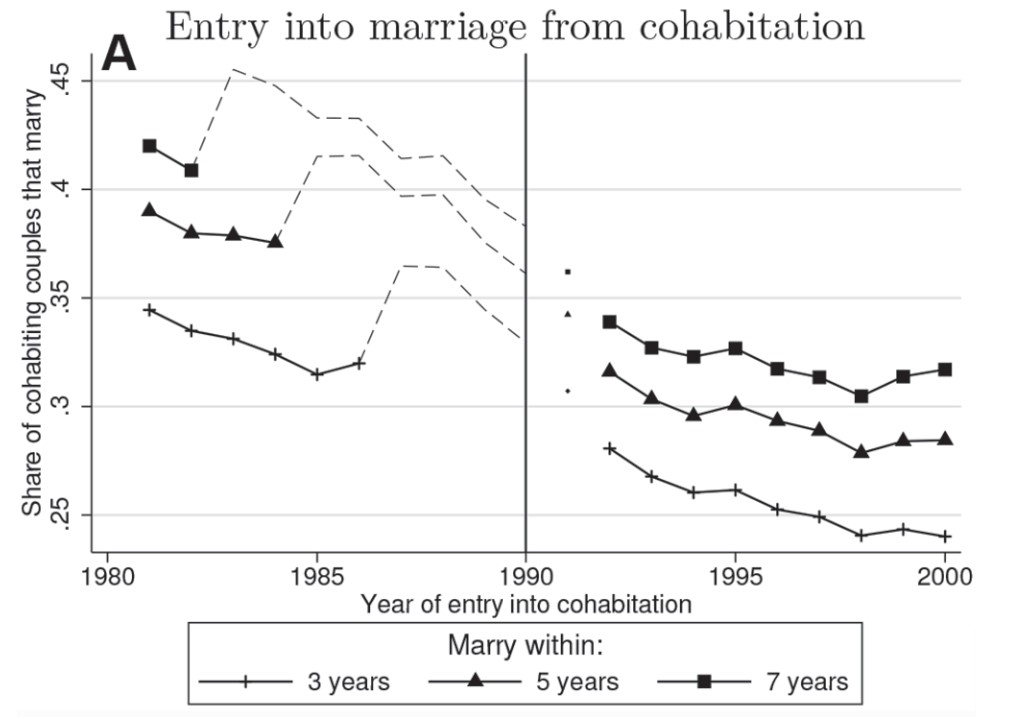
\includegraphics[scale=0.8]{C:/Users/81804/Desktop/readingSummary/figtab/persson_fig2a.jpg}
\caption*{Figure 2A}
\end{figure}

\subsubsection{Steady-state quality of cohabiting unions}
\begin{itemize}
\item Consider only couples that separate within 3, 5, and 7 years after moving in together.
\item Separation rate rises in the long run.
\end{itemize}


\begin{figure}[h!]
\center
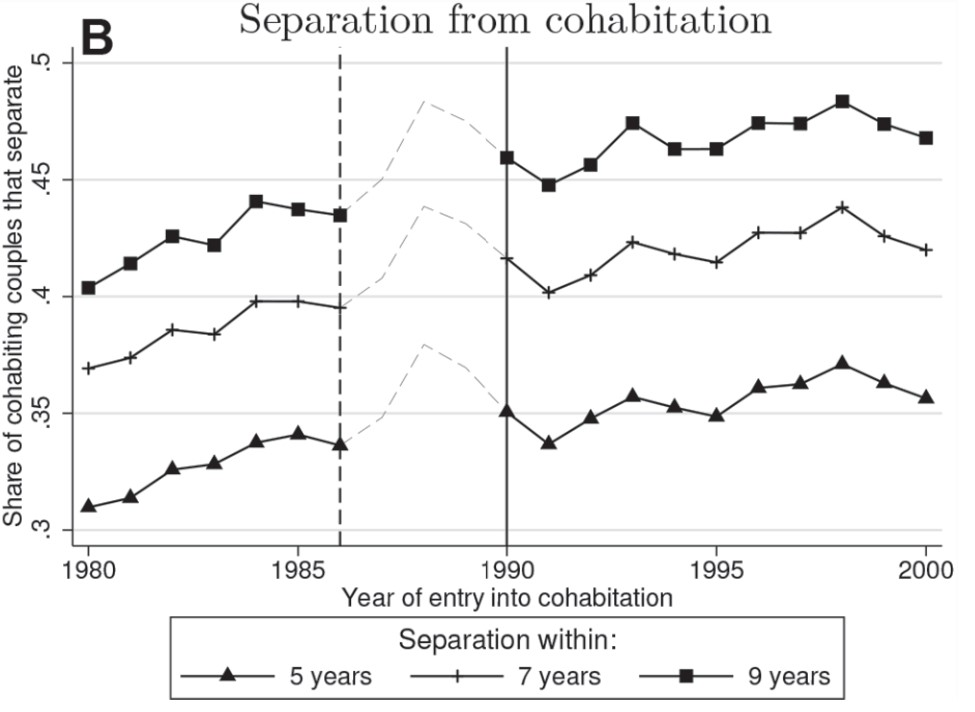
\includegraphics[scale=0.8]{C:/Users/81804/Desktop/readingSummary/figtab/persson_fig2b.jpg}
\caption*{Figure 2B}
\end{figure}

\subsection{Impact around transition period}

\subsubsection{Marriage boom}

\begin{itemize}
\item Figure 3 compares the marriage rate of couples who faced incentive (those with at least one child born before or on December 31, 1989) to marry fast VS those who did not (those whose first joint child was conceived after the elimination of survivors insurance).
\item There is bunching at the quarter right before the reform for those with incentives.
\end{itemize}

\begin{figure}[h!]
\center
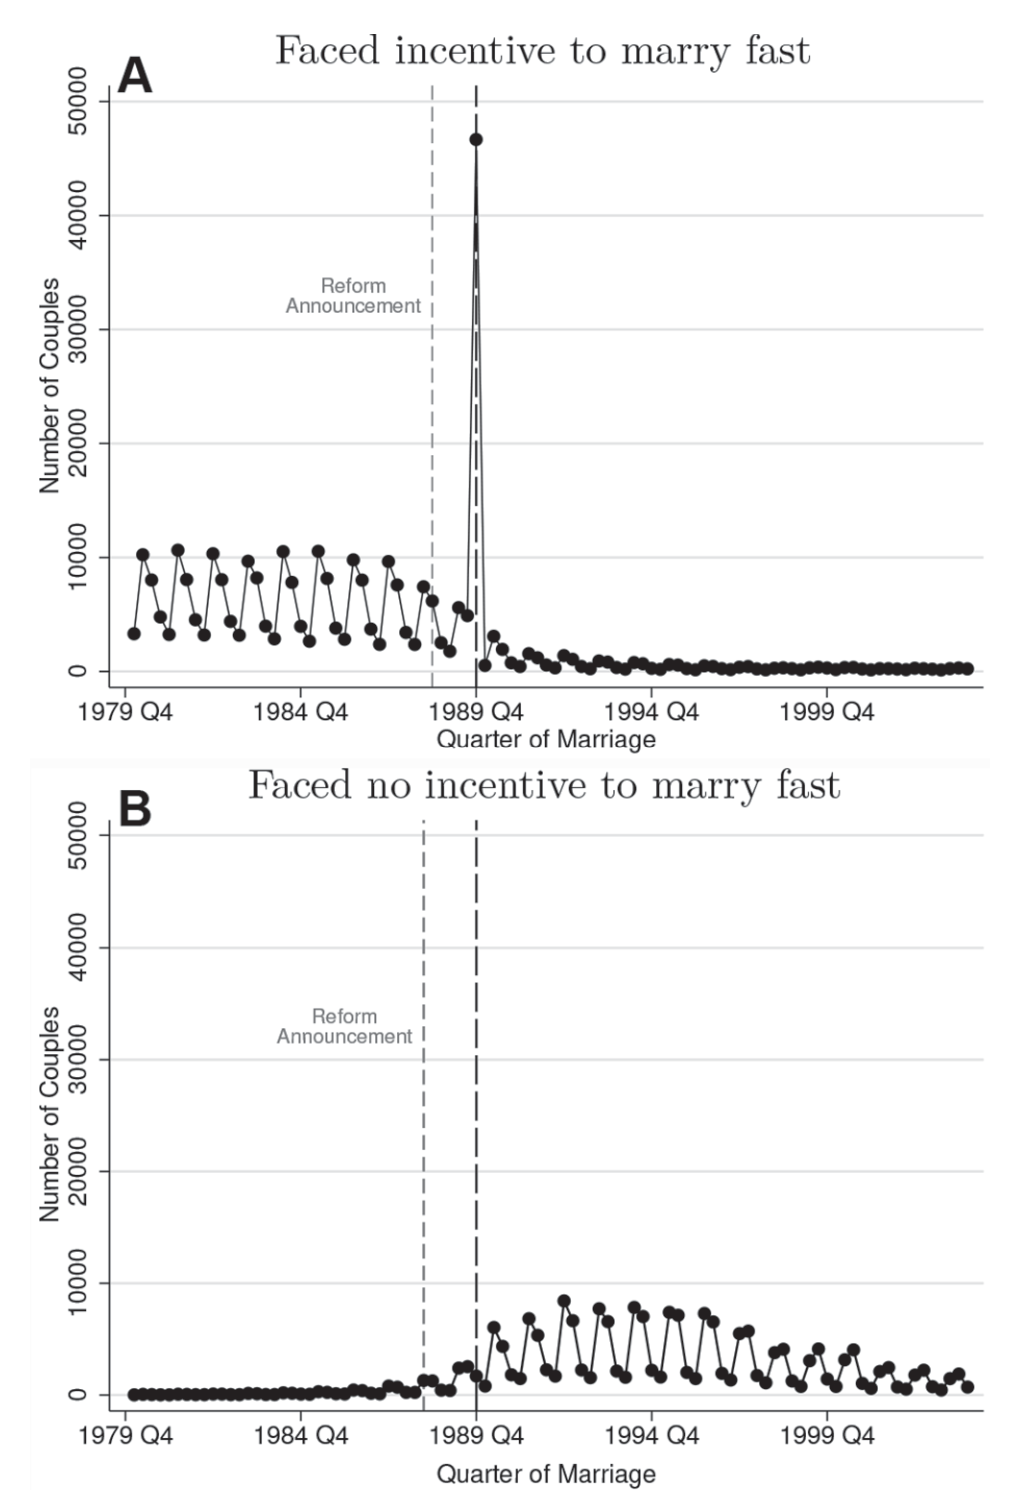
\includegraphics[scale=0.8]{C:/Users/81804/Desktop/readingSummary/figtab/persson_fig3.png}
\caption*{Figure 3}
\end{figure}


\subsubsection{Retimed and Extra marriages}
\begin{figure}[h!]
\center
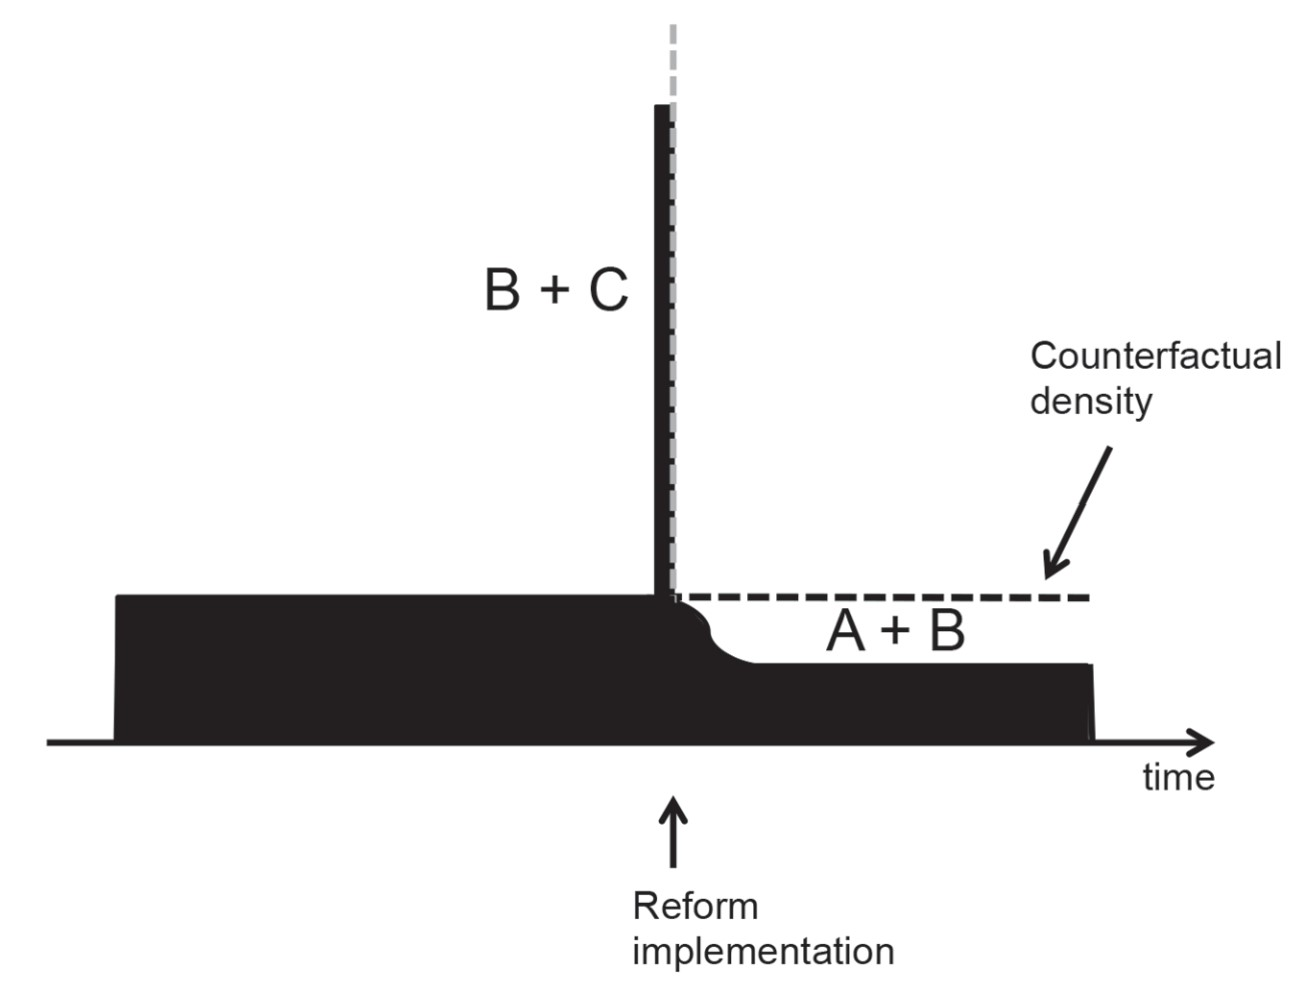
\includegraphics[scale=0.6]{C:/Users/81804/Desktop/readingSummary/figtab/persson_fig4.jpg}
\caption*{Figure 4}
\end{figure}

\begin{itemize}
\item This paper then estimates the effect of the reform by decomposing the time-series plot of marriage over time.
\item Decompose the time series plot into (Figure 4):
\begin{enumerate}
\item Long-run steady state decline of marriage (A)
\item Retimed marriage i.e. marriage that would have occurred after 1989q4 if there was no reform (B)
\item Extra marriage i.e. marriage that would not happen if there was no reform
\end{enumerate}

\item A, B, and C were estimated as follows:
\begin{enumerate}
\item Use two samples:
\begin{itemize}
\item Treated sample: sample with couples with at least one child before the reform. Divide them into 72 cohorts by the time their first child was born (1971q1--1988q4).
\item Untreated sample: sample with couples whose first child was born after the reform. Divide them into 32 cohorts by the time their first child was born (1991q1--1998q4).
\end{itemize}
\item Estimate the following equation
\begin{equation}
n_{cs} = \alpha + \vec{1}[s=s^*]\sum_{c=1}^{72}\beta_c + g(s) + \zeta_q + \eta_c +
 \vec{1}[s>s^*]\sum_{c=1}^{104}\gamma_c + h(t_{prebirth}) + j(t_{postbirth}) + \epsilon_{cs}
\end{equation}
where
\begin{itemize}
\item $\vec{1}[s=s^*]=1$ when period $s$ is $s^*$(1988q4)
\item $\beta_c$ captures bunching at the reform period and is specific to each cohort $c$. $\rightarrow$ B+C
\item $\gamma_c$ captures different things for different samples
\begin{itemize}
\item Treated sample: $\gamma_c$ captures retimed marriage and steady state marriage. $\rightarrow$ B+A
\item Untreated sample: $\gamma_c$ captures steady-state reduction. $\rightarrow$ A
\end{itemize}
\item $g(s)$ is higher-order polynomial in time.
\item $\zeta_q$ and $\eta_c$ are quarter and cohort fixed effects.
\item $h(t_{prebirth})$ and $j(t_{postbirth})$ are higher-order polynomials in the number of quarters before and after the birth of the first child.
\end{itemize}
\item Calculate counterfactuals from treated and untreated samples. Set $\vec{1}[s=s^*]=\vec{1}[s>s^*]=0$ and use $\hat{\alpha}, \hat{\beta}_c, \hat{\gamma}_c, ...$ to get the predicted number of marriages when there is no reform.
\begin{itemize}
\item Untreated sample: We can get A from its counterfactual
\item Treated sample: We can get A+B and B+C from its counterfactual.
\end{itemize}
\item Calculate A, B, and C.
\end{enumerate}
\begin{figure}[h!]
\center
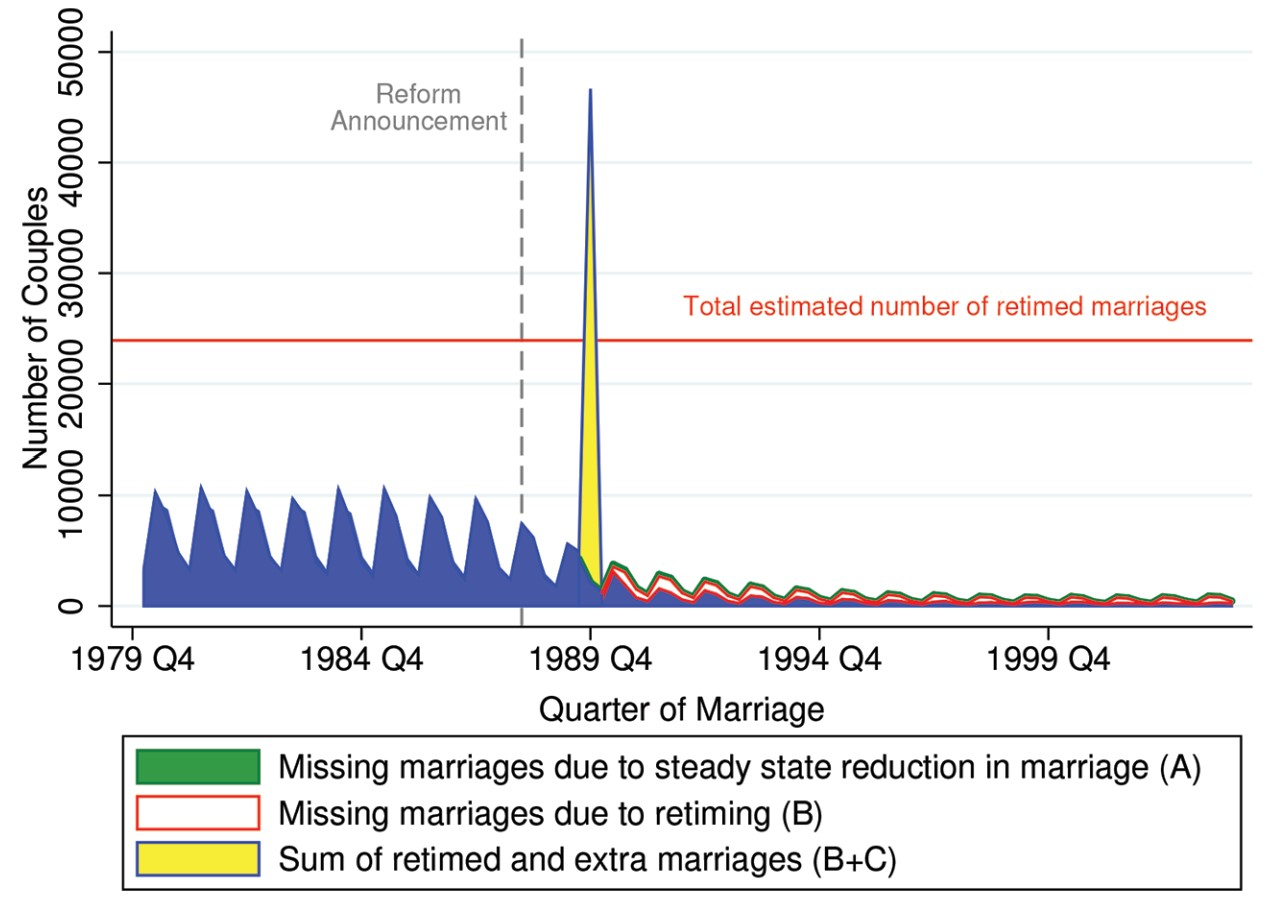
\includegraphics[scale=1]{C:/Users/81804/Desktop/readingSummary/figtab/persson_fig6.jpg}
\caption*{Figure 6}
\end{figure}
\item Identifying assumption: Couples marrying before and after the reform behave the same way when time after childbirth is controlled for.
\end{itemize}

\subsubsection{Heterogeneous effects and economic incentives}

\begin{figure}[h!]
\center
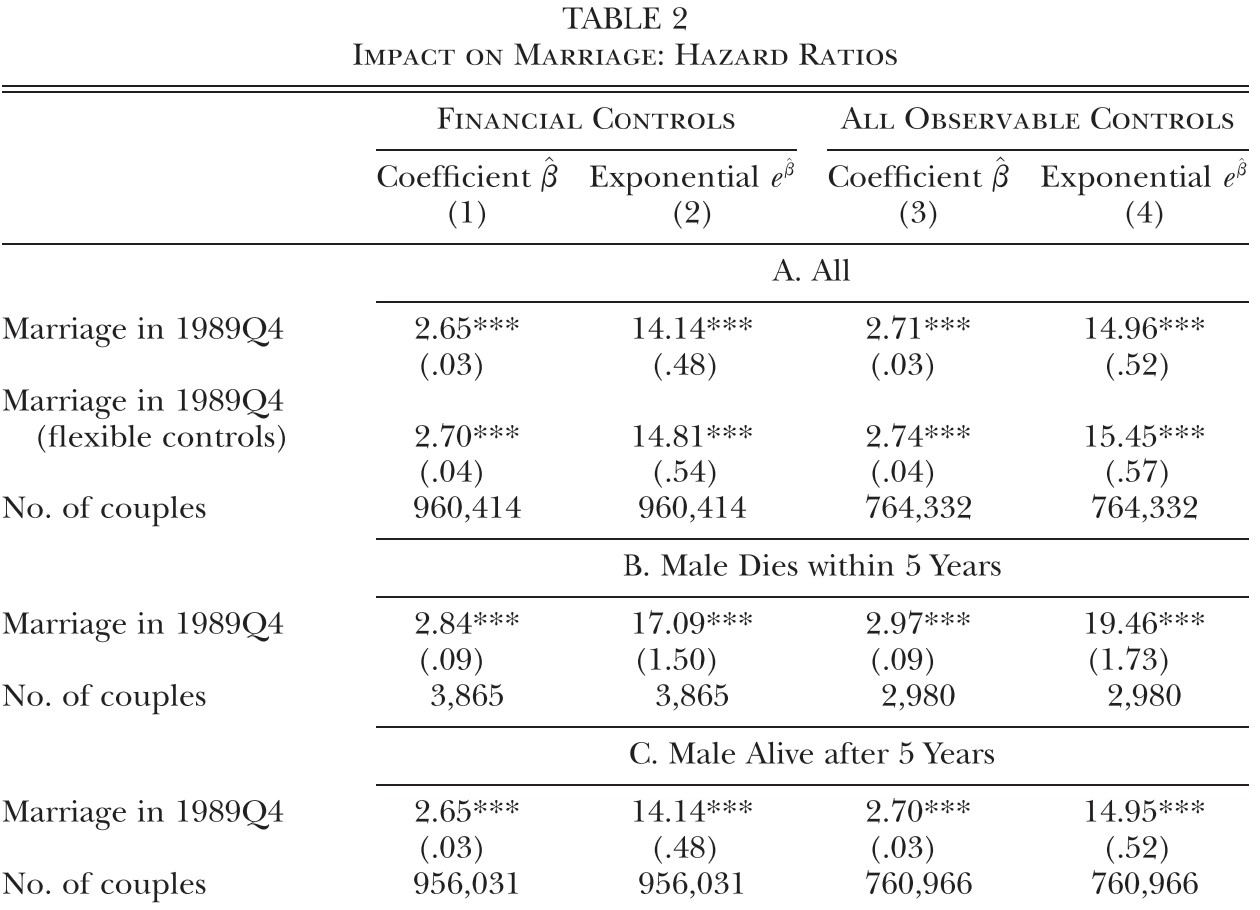
\includegraphics[scale=1]{C:/Users/81804/Desktop/readingSummary/figtab/persson_tab2.jpg}
\caption*{Table 2}
\end{figure}

\begin{itemize}
\item This section analyzes who is likely to marry.
\item It specifies a hazard model that assumes that the risk to enter marriage depends on the first child birth, the reform, and other covariates such as time-varying financial characteristics and couple characteristics. Hazard for marriage at time $t$ is specified as follows:
\begin{equation}
h(t;\vec{Z}_i(t))=h_0(t)\exp(\beta s_i^*(t)+\gamma\text{post}_i(t)+\delta_1 \vec{F}_i(t)+\delta_2\vec{D}_i(t))
\end{equation}

\begin{itemize}
\item $s_i^*(t)=1$ if $t=1989Q4$
\item $\text{post}_i(t)=1$ if $t>1989Q4$
\item $\vec{F}_i(t)$ captures financial characteristics
\item $\vec{D}_i(t)$ captures couple characteristics
\end{itemize}

Only treated sample (couples who have at least one child before the reform) is used. It is assumed that a couple enters the risk pool for marriage 7 years before the birth of the first child.

\item After that, the predicted probability for marriage in 1989Q4 is calculated: $\hat{h}_{1989Q4}=\exp(\beta)$

\item A couple who is unmarried by 1989Q3 is on average 14.14 times more likely to marry in 1989Q4 than they would in the absence of the reform.

\item Next, the author estimates the hazard ratio of each demographic group by adding interactions between male labor income group and age-difference group.

\begin{equation}
h(t;\vec{Z}_i(t))=h_0(t)\exp(\beta s_i^*(t)+\gamma\text{post}_i(t)+\delta_1 \vec{F}_i(t)+\delta_2\vec{D}_i(t))
\end{equation}

\item Figure 8 shows couples are likely to enter marriage in 1989Q4 if the male income is high or age-difference is large.
\end{itemize}

\begin{figure}[h!]
\center
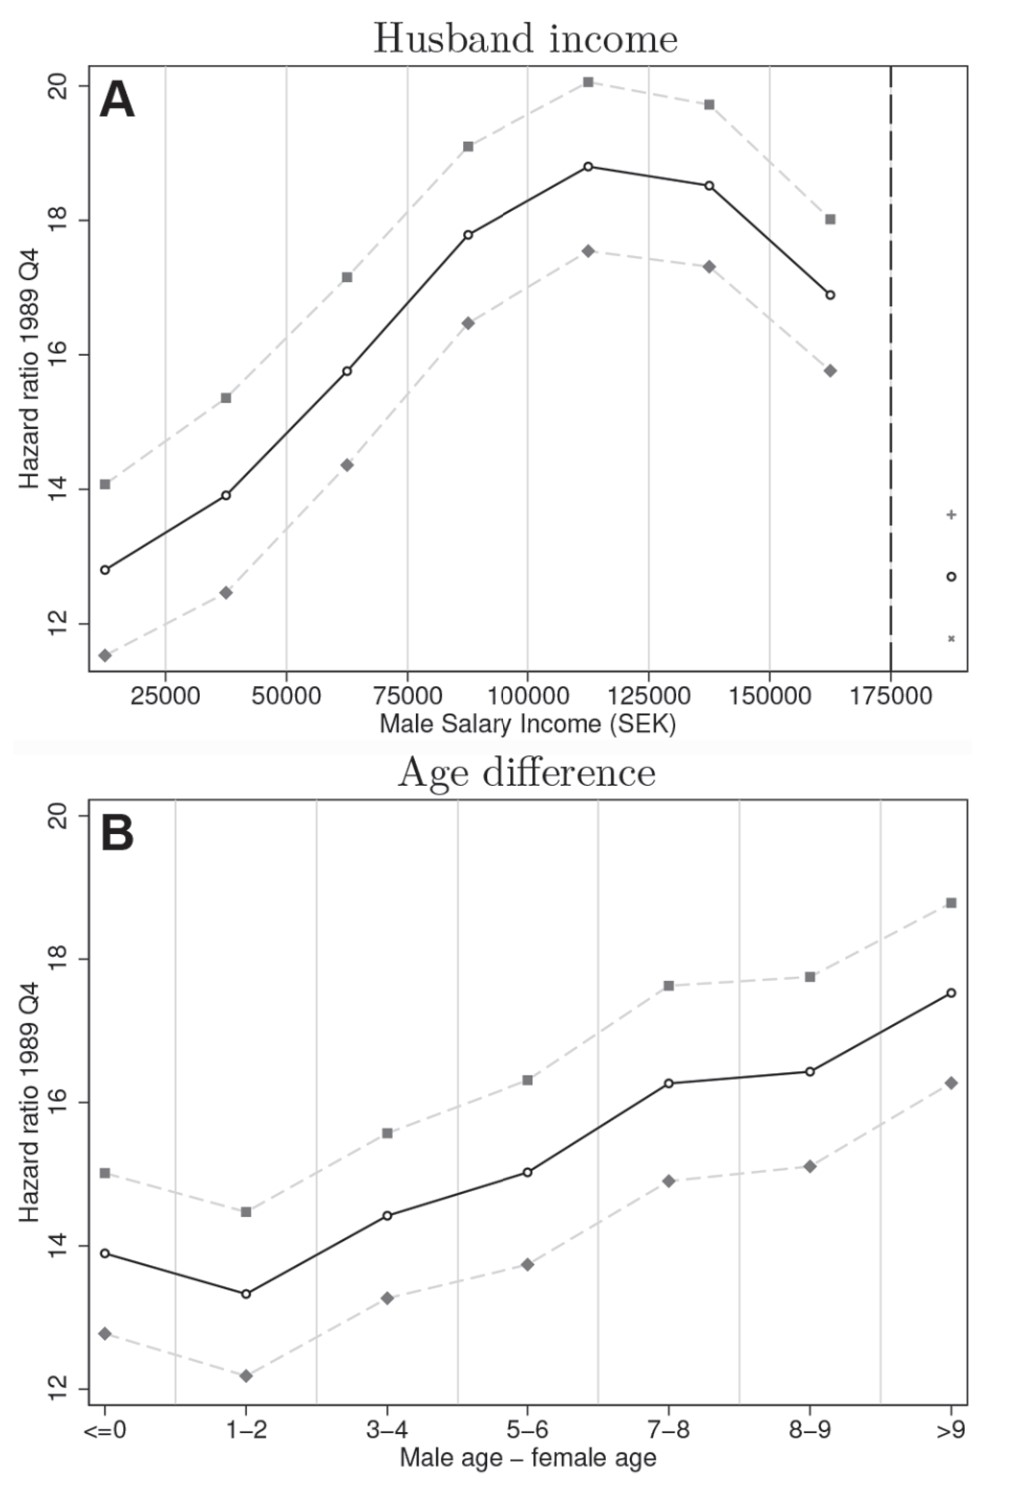
\includegraphics[scale=0.6]{C:/Users/81804/Desktop/readingSummary/figtab/persson_fig8.jpg}
\caption*{Figure 8}
\end{figure}

\subsubsection{Long-run divorce rate in marriages during the boom}

\begin{figure}[h!]
\center
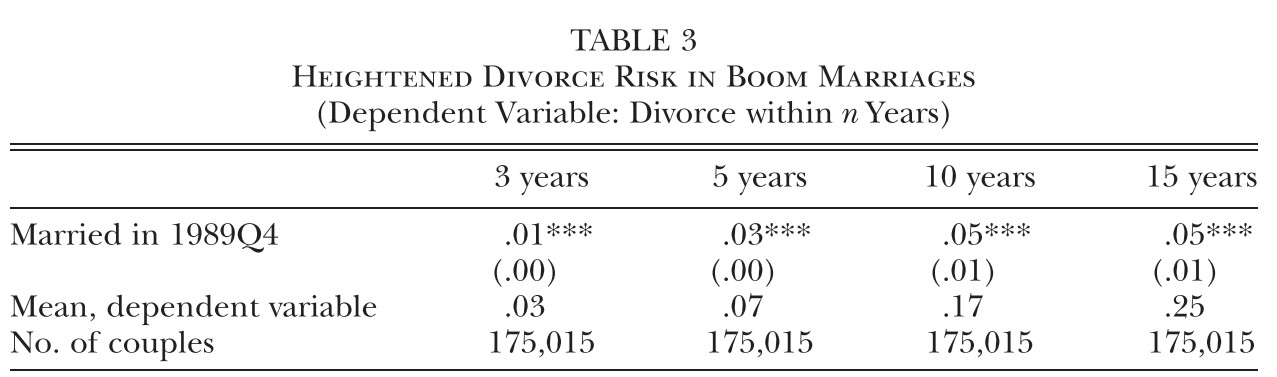
\includegraphics[scale=1]{C:/Users/81804/Desktop/readingSummary/figtab/persson_tab3.jpg}
\caption*{Table 3}
\end{figure}

\begin{itemize}
\item Compare divorce rate within the treated sample of those who marry in 1989Q4 with couples who married earlier. (Table 3)
\end{itemize}

\subsection{Impact on Preexisting Marriages}
\subsubsection{Higher marital instability}
\begin{itemize}
\item This section uses the sample of couples who married in 1984 or 1985 who did not have a joint child. Threshold to the old marriage contract is January 1, 1985. Reform announcement was June 1988.
\item Since marriage date is easily manipulated, couples who marry before and after the New Year's eve may have characteristics that influence marital instability. To address this issue, the author uses DiD combined with RDD. This method captures the difference between two RD estimates: the one within 180 days around January 1, 1984 and the one around January 1, 1985.
\item DiD specification:
\begin{equation}
Y_{it} = \tau_t \times I_{it} + \sigma_t \times \text{NYE}_i + g(dom) + U_{it}
\end{equation}

RD specification:
\begin{equation}
I_{it} = \alpha + \gamma \vec{1}[\tilde{\text{dom}}_b>0]\vec{1}[\text{Around85}]
+\delta\vec{1}[\text{Around85}]
+ g(\tilde{\text{dom}}_b) 
+ h(\tilde{\text{dom}}_b)\vec{1}[\text{Around85}]+\epsilon_{it}
\end{equation}
\begin{itemize}
\item $Y_{it}$: whether the couple $i$ has already divorced in year $t$.
\item $I_t$: survivor insurance status at time $t$
\item $\text{dom}$ : date of marriage
\item NYE : New year's eve
\end{itemize}

\item Result shows the removal of survivors insurance cause divorces after reform announcement in 1988. There is no difference among the placebo groups. (Figure 9)
\end{itemize}

\begin{figure}[h!]
\center
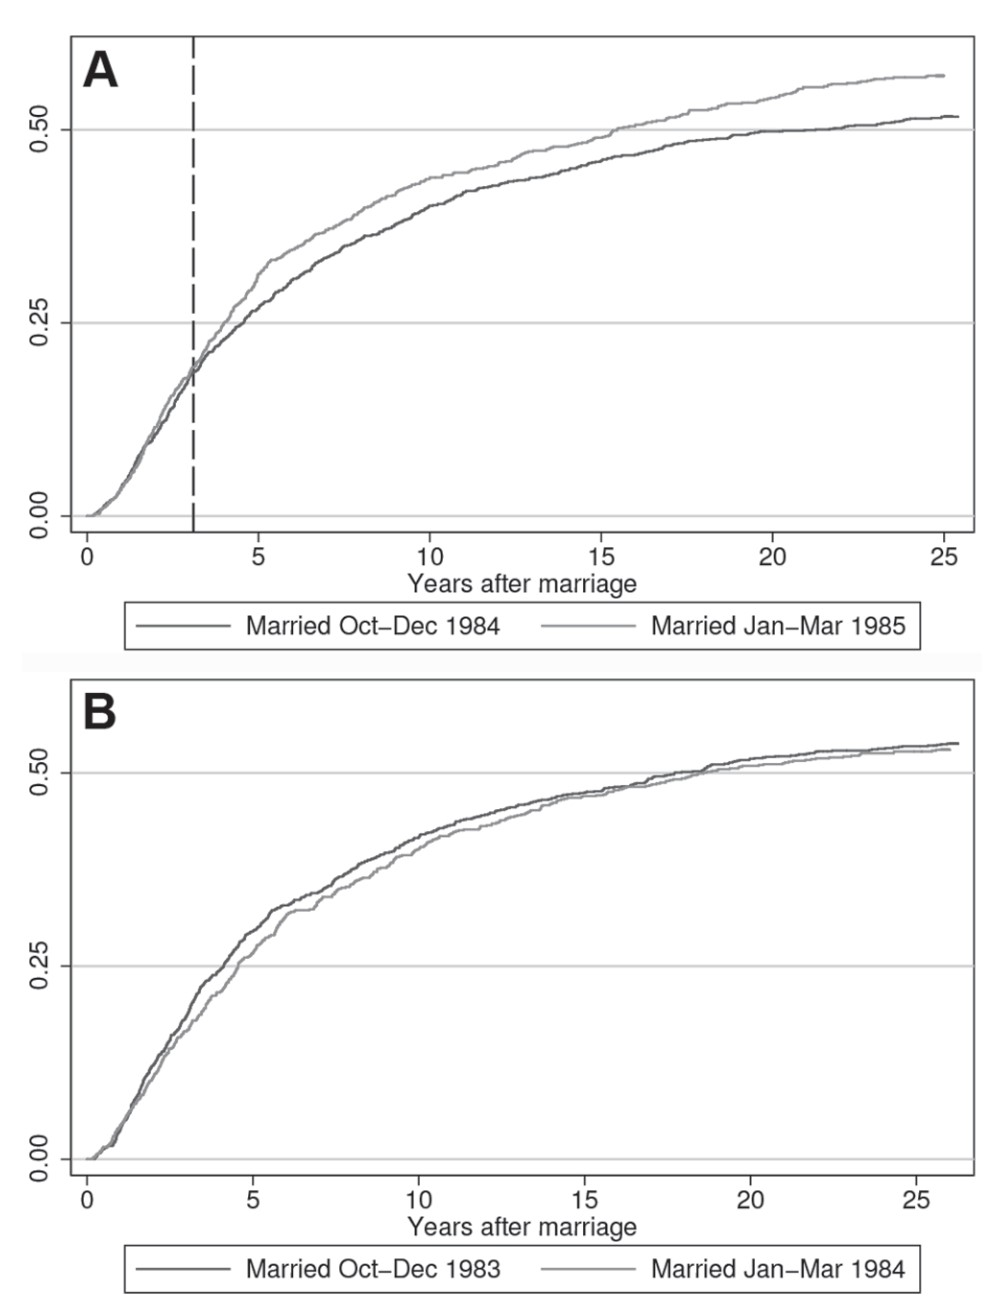
\includegraphics[scale=0.8]{C:/Users/81804/Desktop/readingSummary/figtab/persson_fig9.jpg}
\caption*{Figure 9: CDF of marriage duration}
\end{figure}


\subsection{Impact on Unmatched and Unmarried Individuals}

\subsubsection{Assortativeness of Matching}
\begin{itemize}
\item The old marriage contract favors women who marry men with much higher earnings.
\item Compare the matching patterns of couples who chose to marry in the old VS new marriage contract.
\item The sample includes all couples with children who married from 1983 through 1999. It uses RDD to compare the share of male who married women with less education attainment.
\end{itemize}

\begin{figure}[h!]
\center
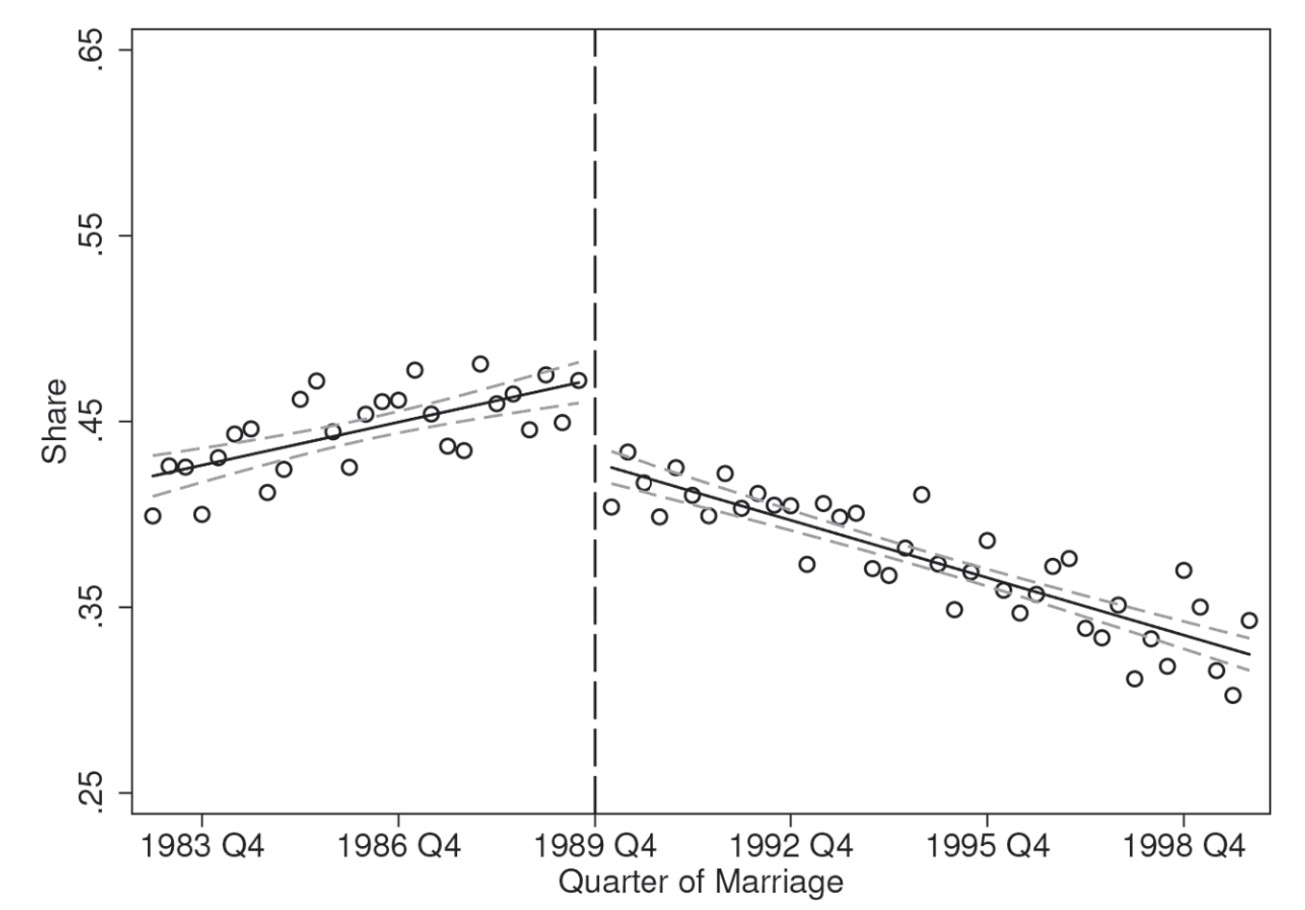
\includegraphics[scale=0.7]{C:/Users/81804/Desktop/readingSummary/figtab/persson_fig10.jpg}
\caption*{Figure 10: CDF of marriage duration}
\end{figure}






\end{document}
